\documentclass{article}

\usepackage[utf8]{inputenc}
\usepackage{enumitem}
\usepackage{multirow}
\usepackage{xcolor}
\usepackage[T1]{fontenc}
% \usepackage[french]{babel}
\usepackage{hyperref}
\usepackage{amssymb}
\usepackage{mathtools}
\usepackage{ntheorem}
\usepackage{amsmath}
\usepackage{amssymb}
\usepackage[ a4paper, hmargin={2cm, 2cm}, vmargin={3cm, 3cm}]{geometry}
\usepackage{capt-of}
\usepackage{multicol}
\usepackage{mathpartir}
\usepackage{stmaryrd}

\usepackage{algorithm}
\usepackage[noend]{algpseudocode}

\usepackage[braket, qm]{qcircuit}
\usepackage{graphicx}

\usepackage{tikz}
\usetikzlibrary{angles,quotes, 3d}

\usepackage{hyperref}
\hypersetup{
    colorlinks,
    citecolor=black,
    filecolor=black,
    linkcolor=blue,
    urlcolor=blue
}

\usepackage{xcolor}

\definecolor{codegreen}{rgb}{0,0.6,0}
\definecolor{codegray}{rgb}{0.5,0.5,0.5}
\definecolor{codepurple}{rgb}{0.58,0,0.82}

\usepackage{listings}
\lstdefinestyle{mystyle}{
    commentstyle=\color{codegreen},
    keywordstyle=\color{magenta},
    numberstyle=\tiny\color{codegray},
    stringstyle=\color{codepurple},
    basicstyle=\ttfamily\footnotesize,
    breakatwhitespace=false,
    breaklines=true,
    captionpos=b,
    keepspaces=true,
    numbers=left,
    numbersep=5pt,
    showspaces=false,
    showstringspaces=false,
    showtabs=false,
    tabsize=2
}
\lstset{style=mystyle}

\theoremstyle{plain}
\theorembodyfont{\normalfont}
\theoremseparator{~--}
\newtheorem*{proof}{Proof}
\newtheorem*{exam}{Example}
\renewcommand\qedsymbol{$\square$}

\newtheorem*{defi}{Definition}
\newtheorem{exo}{Exercise}[section]
\newtheorem{ans}{Answer}[section]
\newtheorem{lemma}{Lemma}[section]
\newtheorem{corr}{Corollary}[section]

\title{Graph Algorithms : Home Assignment}
\author{Valeran MAYTIE}
\date{}

\begin{document}
  \maketitle

  \section*{Exact exponential algorithms for Graph Coloring Problem}

  \begin{enumerate}
    \item The first non-trivial algorithm for 3-Colour.
      \begin{enumerate}
        \item
          Intuitively the root has 3 options then the children are constrained by
          their parents, so they only have 2 as we have a root and n-1 children
          then, there are $3 \times 2^{n-1}$ coloring options.

         We can proof this property by induction on $n$.
          \begin{itemize}
            \item $n=0$, the case where the tree contains no vertex is not
              interesting

            \item $n=1$, if we have one vertex, so we have $3=3\times2^{1-1}$
              3-coloring options

            \item $n+1$, by hypothesis induction, we know that a tree with
              $n$-vertices has $3\times2^{n-1}$ 3-coloring options.

              If we had a vertex on a tree, then it has two possible color
              options, so there is $3\times2^{n-1}\times 2 = 3 \times 2^n$
              3-coloring options.
          \end{itemize}


        \item The 3-coloring algorithm Which uses the \textit{spanning\_tree}
          which returns the spanning tree : $S$. We define \textit{top} and
          \textit{child}, the function who return the top of the tree and the
          child of a vertex. The function return a map with vertex key and color
          (C = $\{c_1, c_2, _3\}$).
          \begin{algorithm}
          \caption{$\mathcal O^*(3^n)$ algorithm for 3-coloring with spanning tree}
          \label{tree_color}
          \begin{algorithmic}[1]
            \Function{rec\_coloring}{G : graph, S: spanning\_tree, v:vertex,
            $\phi$: color}
            \For {$n \in$ \Call{child}{S, v}}
              \State colors = possible\_colors(G, n)
              \For{$c \in $ colors}
                \State $\phi[n] \leftarrow$ c
                \If{\Call{rec\_coloring}{G, S, n, $\phi$}}
                  \State break
                \EndIf
                \State \Return false
              \EndFor
            \EndFor
            \State \Return true
            \EndFunction
            \State
            \Function{3-coloring}{G : graph}
            \State S = \Call{spanning\_tree}{G}
            \State top = \Call{top}{S}
            \State $\phi$ = \{top $\to c_1$\}
            \State \Return \Call{ rec\_coloring}{G, S, top(S), $\phi$}
            \EndFunction
          \end{algorithmic}
          \end{algorithm}
      \end{enumerate}

    \newpage
    \item
      \begin{enumerate}
        \item To reduce to 2-Sat, we want to find clauses containing exactly 2
          literals that allow us to find the colors of the nodes outside
          the dominating set ($X$ : the dominating set and $C$ :
          the set of colors).

          We define the variable:

          $$\mathcal V = \bigcup_{v \in V(G) \backslash X} \{v_c  | \forall c
          \in C\}$$

          All vertices have 3 variables representing if variable $i$ is true then
          the node can have the color $i$.

          We define a function $Cl$ which return a set of clauses for a vertex
          $v$ (represent the possible colors for $v$) :
          \[
            Cl(v) =
            \begin{cases}
              \{(v_1 \vee v_1), (\neg v_1 \vee \neg v_1)\}
              & |\phi(X \cap N_G(v))| = 3  \\
              \{(v_y \vee v_y) | \{y\} = \phi(X \cap N_G(v)) \backslash C\}
              & |\phi(X \cap N_G(v))| = 2 \\
              \{(v_i \vee v_j) | \{i, j\} = \phi(X \cap N_G(v)) \backslash C\}
              & |\phi(X \cap N_G(v))| = 1 \\
            \end{cases}
          \]

          $\phi(X \cap N_G(v))$ is the set of colors link to a vertex $v$.

          The first case is here to make the formula false (we can not choose a
          color if the node is already linked to 3 different colors in $X$).
          In the second case $y$ represent the last color.

          Finally, we define the set $\mathcal C$ of clauses :

          \begin{align*}
            \mathcal C = \bigcup_{v \in V(G) \backslash X} Cl(v) &\cup
            \{(\neg v_c \vee \neg n_c) |\forall n, c \in (N_G(v) \backslash X) \times
            (\phi(X \cap N_G(v)) \backslash C) \} \\
            & \cup \{(\neg v_c \vee \neg v_c) | \forall c \in \phi(N_X(v)\}
          \end{align*}

          The middle union represents the constraints between the external nodes
          of $X$. The last union prevents an external node to have the same
          colors that a neighbor in $X$.

          \textit{Proof :}

          \begin{itemize}
            \item Coloring $\Rightarrow$ 2-Sat :

              We assume that the vertices $V(G) \backslash X$ can be colored.

              We define for all $v$, $v_{c(v)} = true$ and for other color
              $c$ we define $v_c = false$.

              All clauses generated by $Cl$ are
              satisfied (the first case does not occur because the graph can be
              colored).

              We need to make a case disjunction for the other
              clauses of the form $(\neg v_c \vee \neg n_c)$.
              If we have $v_c = true$ then $v$ has the color $c$ has the color
              $c$ and $n$ cannot
              have the color $c$ because they are neighbors, then $n_c = false$.
              Otherwise, $v$ has not the color $c$, so $v_c = false$.

              Finally, the clauses of the form $(v_c \wedge v_c)$ (last union)
              is true because $v$ is linked to a vertex in $X$ which has the
              color $c$, so $v(x) \not = c$.

            \item 2-Sat $\Rightarrow$ Coloring :

              We assume that the formula for a dominating set $X$ is
              satisfiable.

              So we have for all variable $v$ in $V(G)\backslash X$ a $c$ such
              that $v_c = true$, thanks to the function $Cl$.

              The same vertex
              $v$ has no neighbor $n$ such that $n_c = true$. Because we have
              the clause $(\neg v_c \vee \neg n_c)$, if $v_c = true$ then $n_c =
              false$.

              And thanks to the last union we can not have $v_c$ is $v$ is
              linked to a vertex who has the color $c$ in $X$.
          \end{itemize}

          \newpage
          \textit{Example :} $C = \{R, G, B\}$ (R : Red, G : Green, B : Blue)

          \begin{center}
          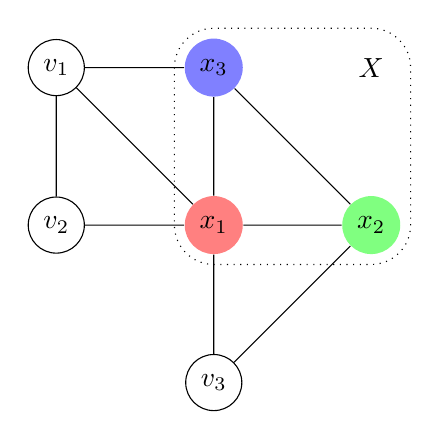
\begin{tikzpicture}
            \node[circle, fill=red!50  ](X1) at (0,0) {$x_1$};
            \node[circle, fill=green!50](X2) at (2,0) {$x_2$};
            \node[circle, fill=blue!50 ](X3) at (0,2) {$x_3$};
            \node at (2, 2) {$X$};
            \draw (X1) -- (X2) -- (X3) -- (X1);
            \draw[dotted, rounded corners=0.5cm]
              (-0.5, 2.5) rectangle (2.5, -0.5);
            \node[draw, circle](V1) at (-2,2) {$v_1$};
            \node[draw, circle](V2) at (-2,0) {$v_2$};
            \node[draw, circle](V3) at (0,-2) {$v_3$};
            \draw (V1) -- (X3) (V1) -- (X1) -- (V2) (V1) -- (V2)
                  (V3) -- (X2) (V3) -- (X1) -- (V3);
        \end{tikzpicture}
        \end{center}

          For this graph we have the formula :

        \begin{align*}
          &(v_{1_G} \vee v_{1_G}) \wedge (\neg v_{1_B} \vee \neg v_{1_B}) \wedge
          (\neg v_{1_R} \vee \neg v_{1_R}) \wedge (\neg v_{1_G} \vee \neg v_{2_G})
          \wedge \\
          &(v_{2_G} \vee v_{2_B}) \wedge (\neg v_{2_R} \vee \neg v_{2_R})
          \wedge (\neg v_{2_G} \vee \neg v_{1_G})
          \wedge (\neg v_{2_B} \vee \neg v_{1_B}) \wedge \\
          &(v_{3_B} \vee v_{3_B}) \wedge (\neg v_{3_R} \vee \neg v_{3_R})
          \wedge (\neg v_{3_G} \vee \neg v_{3_G})
        \end{align*}

        Now, we can construct $c : V(G) \to [3]$. If the formula is not
        satisfiable then $c$ can not be constructed. Otherwise, we can define
        $c$ like that :

        \[
          c(x) =\begin{cases}
            \phi(x) & \text{if } x \in X \\
            c \hspace{1cm} x_c = \text{true}
          \end{cases}
        \]

        If the formula is satisfiable we necessarily have $c$ such that $x_c =
        true$ (by construction).

      \item Let $G$ a graph such as $V(G) \geq 2$ and $T$ the corresponding BFS
        tree. We have $S_i$ the set of vertices at layer $i$ of tree $T$.

        We define the sets $D_e = \{v | v \in S_i, \exists k, i = 2 \times k\}$
        (vertices in an even layer) and \\
        $D_o = \{v | v \in S_i, \exists k, i = 2 \times k + 1\}$ (vertices in an
        odd layer).

        $D_e$ and $D_o$ are distinct sets because in a BFT tree we can not have
        the same vertex several times, so the layer where the even and odd
        layers intersect is empty.

        $D_e$ De is a dominating set, because each layer is linked to
        the layer below and above it, so it is linked to all the other
        remaining vertices. We apply the same argument to $D_o$.

        We can deduce that the upper bound of the smallest dominating set is
        $\frac n 2$ ($n = |V(G)|$). If $|D_e| < |D_o|$, then the smallest is
        $D_e$ otherwise the smallest is $D_o$.
        So the worst case is when $|D_e| = |D_o| = \frac n 2$.

        \textit{Example :}
        \begin{center}
        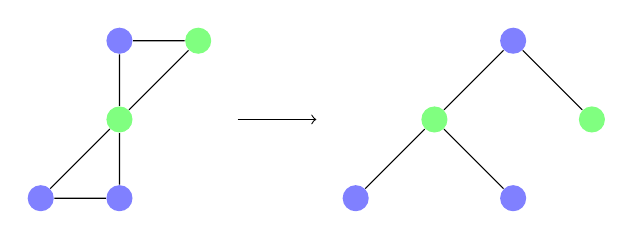
\begin{tikzpicture}
          \node[circle, fill=blue!50 ](G1) at ( 0, 0) { };
          \node[circle, fill=green!50](G2) at ( 1, 0) { };
          \node[circle, fill=green!50](G3) at ( 0,-1) { };
          \node[circle, fill=blue!50 ](G4) at (-1,-2) { };
          \node[circle, fill=blue!50 ](G5) at ( 0,-2) { };

          \draw (G1) -- (G2) -- (G3) -- (G4) -- (G5) -- (G3) -- (G1);

          \node[circle, fill=blue!50 ](G1) at (5, 0) { };
          \node[circle, fill=green!50](G2) at (4,-1) { };
          \node[circle, fill=green!50](G3) at (6,-1) { };
          \node[circle, fill=blue!50 ](G4) at (3,-2) { };
          \node[circle, fill=blue!50 ](G5) at (5,-2) { };
          \draw (G1) -- (G2) -- (G4) (G2) -- (G5) (G1) -- (G3);

          \draw[->] (1.5, -1) -- (2.5, -1);
        \end{tikzpicture}
        \end{center}

      \item
        The \textit{BFS\_tree}, \textit{bi\_party} and \textit{2-Sat}
        functions have a polynomial complexity. We use \textit{3-coloring}
        (Algorithm-\ref{tree_color}) on a graph such that $|V(G)| = \frac n 2$,
        then the complexity is $\mathcal O^* (3^{\frac n 2}) = \mathcal
        O^*((\sqrt 3)^n)$. Therefor, the algorithm below has a complexity of
        $\mathcal O^*((\sqrt3)^n)$.

        \begin{algorithm}
          \caption{$\mathcal O^*((\sqrt 3)^n)$ algorithm for 3-coloring with the
          smallest dominating set}
          \label{sqrt3}
          \begin{algorithmic}[1]
            \Function{3-coloring-opt}{$G$ : graph}
              \State $T$ = \Call{BFS\_tree}{$G$}
              \State $D_e$, $D_o$ = \Call{bi\_party}{$T$}
              \State $X$ = $D_e$
              \If{$|D_o| < B$}
              \State $X \leftarrow D_o$
              \EndIf
              \State $\phi$ = \Call{3-coloring}{$X$}
              \State $\phi \leftarrow$ \Call{2-Sat}{$G$, $X$, $\phi$}
            \EndFunction
          \end{algorithmic}
          \end{algorithm}
      \end{enumerate}

    \newpage
    \item
      \begin{enumerate}
        \item We have $X \subseteq V(G)$ and $1 \leq j < k$ such that
          $\chi(G[X]) \leq j$. We want to compute $Y \subseteq V(G)$ such that
          $\chi(G[Y]) \leq j + 1$. The function $\mathcal P(X)$ give all
          possible subset of a set $X$. So for all $S \in \mathcal P (V(G))$
          if $S$ is on $X$ then $\chi(G[S]) \leq j \leq j + 1$. Otherwise,
          if we find $S_p \in \mathcal P(S)$ such as $S_p \in X$ ($\phi_p$,
          $j$-coloring of $S_p$) and $\phi$ such that $\phi(x) = \phi_p(x)$ if
          $x \in S_p$ else $\phi(x) = j + 1$ is a $j+1$-coloring of $S$, then
          $S$ is in $Y$.

          For all subset we have to potentially calculate all the subset of a
          subset of cardinal $t$($\mathcal O^*(2^n))$. We did this operation
          for all the subsets of vertices in the graph.

          So we have a complexity of

          $$\sum_{t=0}^n \binom n t \mathcal O^*(2^t) = \mathcal O^*(3^n)$$

      \item The final algorithm :

        \begin{algorithm}
          \caption{$\mathcal O^*(3^n)$ algorithm for k-coloring}
          \begin{algorithmic}[1]
            \Function{k-coloring}{$G$ : graph}
              \State k = 0
              \State X = \{\}
              \While{$V(G)$ not in M}
                \State k = k + 1
                \ForAll{$C \subseteq V(G)$}
                  \If{$C \in $ X}
                    \State Continue
                  \EndIf
                  \ForAll{$S \subseteq C$}
                    \If{$S \not \in$ X}
                    \State Continue
                    \EndIf
                    \State $\phi_s$ = X[S] $\cup \{v \to k| \forall v \in C
                      \backslash S\}$
                    \If{\Call{is\_coloring}{$C$, $\phi_s$}}
                      \State X[C] $\leftarrow \phi_s$
                      \State Break
                    \EndIf
                  \EndFor
                \EndFor
              \EndWhile
              \State \Return k
            \EndFunction
          \end{algorithmic}
          \end{algorithm}

          The algorithms above finished, because a graph always has a colouring
          ($\leq n$). It repeats the algorithm detailed in the previous question
          at most $n$ times, so it has a complexity of $\mathcal O^*(3^n)$.

          The dictionary $X$ containing, at worst, all the parts of the set of
          vertices. So the space complexity is $\mahtcal O^*(2^n)$
      \end{enumerate}
  \end{enumerate}

\end{document}
